\chapter{代码插入与劫持技术分析}



%%%%%%%%%%%%%%%%%
%%%%%% 2.1%%%%%%%
%%%%%%%%%%%%%%%%% 

%\section{代码插入与劫持技术的应用}



%%%%%%%%%%%%%%%%
%%% 2.2 %%%%%%%%
%%%%%%%%%%%%%%%% 

\section{关于ELF格式的讨论}

对ELF格式文件进行二进制层面的修改,
首先要对其文件格式有比较深入的了解。
ELF的文件格式在\cite{elf1.2}中有着详尽的描述,
在此不再对ELF文件格式的细节进行罗列,
而是介绍一些关键的知识,
并讨论这些知识与我们的插入工作有何关联,
以及它们如何能决定插入的成败。

  \subsection{ELF文件类型} 

ELF文件主要有三种类型,分别是:

\begin{itemize}
 \item 可重定位文件(Relocatable File)
 \item 可执行文件(Executable File)
 \item 共享目标文件(Shared Object File)
\end{itemize}

可重定位文件就是常见的.o文件,也叫目标文件。
这类文件包含了代码和数据,
但是其中的外部地址引用都未重定位,
可以被与其他可重定位文件链接生成
可执行文件或者共享目标文件。

可执行文件在Linux下往往没有扩展名,
例如/bin/ls就是典型的这一类文件。
他们共同的特点是可以直接执行。
但是ELF可执行文件在也分为两类:
静态链接的和动态链接的。
区别在于静态链接的文件所需要的库都已经被链接至
可执行文件中。而动态链接的文件在运行时才与库链接。
Gcc(GNU Compile Collection, GNU编译器套装)默认生成动态链接的可执行文件;通过增加--static选项,可以生成静态链接的可执行文件。

共享目标文件即Linux下的.so文件,
也常被叫做动态共享库。
它们类似.o文件,并没有被完全链接,
但是区别在于,
它们用于在运行时与动态链接的可执行文件进行链接。

我们的操作目标,即VxWorks系统镜像,
可以归类为静态链接的可执行文件。
它的特点是已经被完全链接和重定位。

\subsection{链接视图与执行视图}

每一种ELF文件都有着相似的基础结构。
ELF文件格式刚刚被生成的时候,是存储在磁盘中;
然而它最终的用途是被加载和执行。
这里有点类似从一个“程序”到“进程”的转化。
当ELF存在于磁盘中时,系统以某种视角来看待它;
然而当它被加载到主存,系统就需要以另一种视角来看待它。
%%
这两种不同的视角,
就是ELF文件的链接视图和执行视图,
如图\ref{elf-map}。
任何ELF文件都存在链接视图,
而执行视图存在于共享目标文件和可执行文件中。

\begin{figure}[h!]
  \centering
  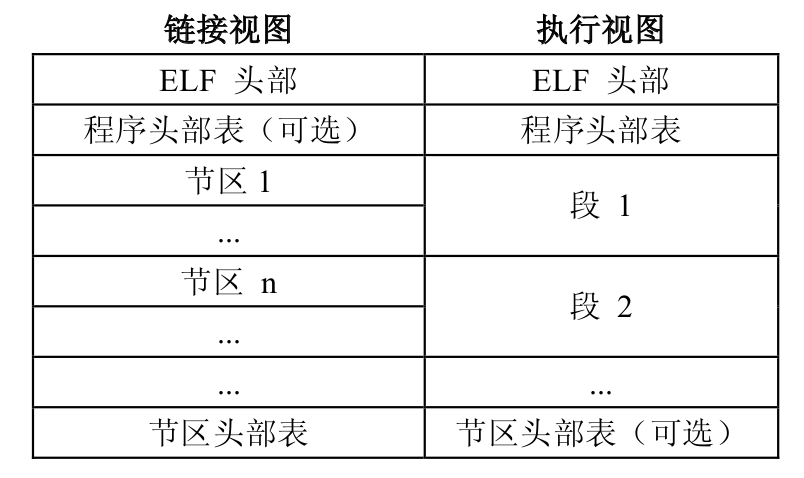
\includegraphics[width=0.55\textwidth]{figure/elf-map.png}
  \caption{链接视图与执行视图}
  \label{elf-map}
\end{figure}

\begin{itemize}
  \item 链接视图
\end{itemize}

在对ELF文件进行链接的过程中,
链接器从链接视图来看待ELF文件,
链接器认为ELF文件被划分为一个个节区(section),
节区中包含代码或者数据。
链接器通过合并这些段来形成新的ELF文件。

\begin{itemize}
  \item 加载视图
\end{itemize}


当加载器对ELF可执行文件执行加载操作时,
它眼中的ELF文件是被划分为了一个个段(segmentation)。
在一个使用分页机制的系统中,
每个段都是按照页大小(例如4KB)进行对齐的。
加载器的任务就是把每个段的页拷贝到主存的合适位置。
(使用虚拟存储器的系统中,加载器不拷贝数据,
只建立虚拟内存和磁盘文件的关联,
在此可以简单认为加载器按照段结构进行了ELF文件到主存的拷贝)

ELF文件中,存在以下的数据结构,来实现链接视图和执行视图。
(在.o文件中,不存在执行视图)

\begin{itemize}
  \item 节区与节区头部表
\end{itemize}

图\ref{sections}展示了/bin/ls程序的节区头部表的一部分。
在链接视图中,节区用于划分文件中不同类型的数据。
例如.text节用于存放代码,.data节用于存放数据等。
链接两个目标文件的的其中一步,就是把
节区头表为是所有节区的一个索引,
通过解析节区头表可以找到文件的所有节区。

%%\begin{lstlisting}[
%% language={C},
%% label={sections},
%%caption={节区头部表},
%%xleftmargin=2em,xrightmargin=2em, aboveskip=1em,
%%]
%%Section Headers:
%%  [Nr] Name              Type            Addr     Off    Size   ES Flg Lk Inf Al
%%  [ 0]                   NULL            00000000 000000 000000 00      0   0  0
%%  [ 1] .interp           PROGBITS        08048154 000154 000013 00   A  0   0  1
%%  [ 2] .note.ABI-tag     NOTE            08048168 000168 000020 00   A  0   0  4
%%  [ 3] .note.gnu.build-i NOTE            08048188 000188 000024 00   A  0   0  4
%%  [ 4] .gnu.hash         GNU_HASH        080481ac 0001ac 00006c 04   A  5   0  4
%%  [ 5] .dynsym           DYNSYM          08048218 000218 000820 10   A  6   1  4
%%  [ 6] .dynstr           STRTAB          08048a38 000a38 0005d5 00   A  0   0  1
%%  [ 7] .gnu.version      VERSYM          0804900e 00100e 000104 02   A  5   0  2
%%  [ 8] .gnu.version_r    VERNEED         08049114 001114 0000d0 00   A  6   3  4
%%  [ 9] .rel.dyn          REL             080491e4 0011e4 000038 08   A  5   0  4
%%  [10] .rel.plt          REL             0804921c 00121c 000380 08   A  5  12  4
%%  [11] .init             PROGBITS        0804959c 00159c 000023 00  AX  0   0  4
%%  [12] .plt              PROGBITS        080495c0 0015c0 000710 04  AX  0   0 16
%%  [13] .text             PROGBITS        08049cd0 001cd0 010fcc 00  AX  0   0 16
%%  [14] .fini             PROGBITS        0805ac9c 012c9c 000014 00  AX  0   0  4
%%  [15] .rodata           PROGBITS        0805acc0 012cc0 0040c8 00   A  0   0 32
%%  [16] .eh_frame_hdr     PROGBITS        0805ed88 016d88 00072c 00   A  0   0  4
%%  [17] .eh_frame         PROGBITS        0805f4b4 0174b4 0028b8 00   A  0   0  4
%%  [18] .init_array       INIT_ARRAY      08062eec 019eec 000004 00  WA  0   0  4
%%  [19] .fini_array       FINI_ARRAY      08062ef0 019ef0 000004 00  WA  0   0  4
%%  [20] .jcr              PROGBITS        08062ef4 019ef4 000004 00  WA  0   0  4
%%  [21] .dynamic          DYNAMIC         08062ef8 019ef8 000100 08  WA  6   0  4
%%  [22] .got              PROGBITS        08062ff8 019ff8 000008 04  WA  0   0  4
%%  [23] .got.plt          PROGBITS        08063000 01a000 0001cc 04  WA  0   0  4
%%  [24] .data             PROGBITS        080631e0 01a1e0 000160 00  WA  0   0 32
%%  [25] .bss              NOBITS          08063340 01a340 000c64 00  WA  0   0 32
%%  [26] .gnu_debuglink    PROGBITS        00000000 01a340 000008 00      0   0  1
%%  [27] .shstrtab         STRTAB          00000000 01a348 0000fc 00      0   0  1
%%Key to Flags:
%%  W (write), A (alloc), X (execute), M (merge), S (strings)
%%  I (info), L (link order), G (group), T (TLS), E (exclude), x (unknown)
%%  O (extra OS processing required) o (OS specific), p (processor specific)
%%\end{lstlisting}

\begin{figure}[h!]
  \centering
  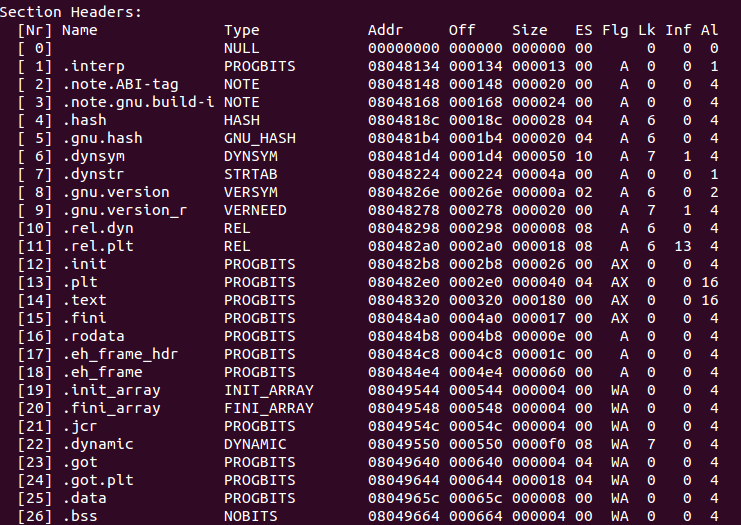
\includegraphics[width=0.85\textwidth]{figure/sections.png}
  \caption{节区头部表}
  \label{sections}
\end{figure}

\begin{itemize}
  \item 段和程序头部表
\end{itemize}

图\ref{programs}是/bin/ls的程序头部表。
段是执行视图中的对ELF文件的划分,
ELF文件被加载和执行的就是一个个段。
一般来说,每个节区映射到唯一一个段,而一个段包含不同的节区。
段没有名字,但有类型和属性:
类型一般指明该段是否需要加载至内存,
例如需要加载器加载到主存中的段的类型为“LOAD”;
而段的属性则表明了该段能否被读/写/执行。

%%\begin{lstlisting}[
%%caption={程序头部表},
%%language={C},
%% label={programs},
%%xleftmargin=2em,xrightmargin=2em, aboveskip=1em,
%%]
%%Program Headers:
%%  Type           Offset   VirtAddr   PhysAddr   FileSiz MemSiz  Flg Align
%%  PHDR           0x000034 0x08048034 0x08048034 0x00120 0x00120 R E 0x4
%%  INTERP         0x000154 0x08048154 0x08048154 0x00013 0x00013 R   0x1
%%      [Requesting program interpreter: /lib/ld-linux.so.2]
%%  LOAD           0x000000 0x08048000 0x08048000 0x19d6c 0x19d6c R E 0x1000
%%  LOAD           0x019eec 0x08062eec 0x08062eec 0x00454 0x010b8 RW  0x1000
%%  DYNAMIC        0x019ef8 0x08062ef8 0x08062ef8 0x00100 0x00100 RW  0x4
%%  NOTE           0x000168 0x08048168 0x08048168 0x00044 0x00044 R   0x4
%%  GNU_EH_FRAME   0x016d88 0x0805ed88 0x0805ed88 0x0072c 0x0072c R   0x4
%%  GNU_STACK      0x000000 0x00000000 0x00000000 0x00000 0x00000 RW  0x4
%%  GNU_RELRO      0x019eec 0x08062eec 0x08062eec 0x00114 0x00114 R   0x1
%%}
%%\end{lstlisting}

\begin{figure}[h!]
  \centering
  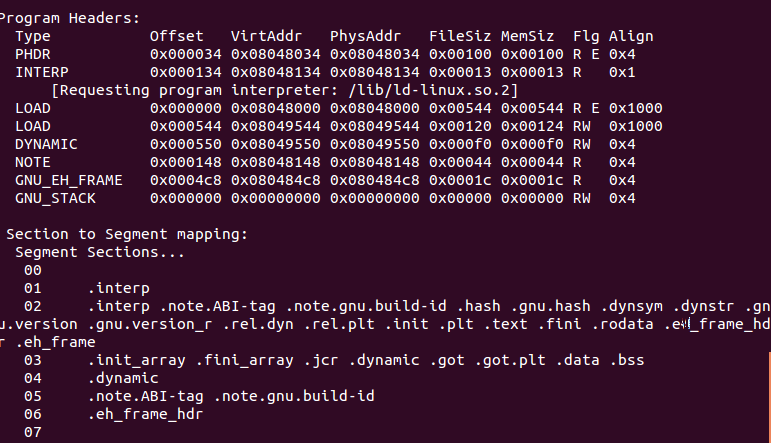
\includegraphics[width=0.85\textwidth]{figure/programs.png}
  \caption{程序头部表}
  \label{programs}
\end{figure}

在一个典型的Linux可执行文件中,
第一个LOAD类型的段一般具有可读和可执行的属性,
该段对应的节区为所有含有代码的节区,例如.init节、.text节和.finit节。

与节区头部表类似,程序头部表是所有段的一个索引。
程序头部表还指明了每个段所包含的节区。

\subsection{文件空间和地址空间}
\label{twoqs}
上文介绍了ELF文件的两种不同的视图,
理解两个视图的区别和联系能帮助我们找到可以插入代码的位置。
然而,这还是不够的。
我们插入的代码必须加载到一定的地址才能被运行。
这就需要理解ELF文件与地址空间的关系。

在节区头部表和程序头部表中,
不但指定了节区或者段在文件中的位置,
还指定了节区或者段在内存中的加载地址。
例如如图\ref{sections}所示,
/bin/ls程序包含的.text节在文件中的偏移是0x3020,
而加载地址为0x8048320。

打个比方,如果在论文中新加入了一个章而没有更新目录,
那么这一章很可能会被读者忽略。
类似地,在ELF文件中插入代码,如果不更新相应的数据结构(节头表和程序头表),
除了增大了文件的体积之外和导致文件不能运行之外,
没有任何意义。

由于插入的代码会影响文件内容在文件中的偏移,
因此相应节头表和段表的偏移字段必须被更新。
如果这项工作没有出现错误,
那么修改后的文件至少是可以正常地像原先一样执行的。
然而,要让我们插入的代码也在加载时被映射到
程序的地址空间中,那插入的部分必须拥有合法的载入地址。

这就带来了两个问题,一是哪些地址空间是空闲并可以使用的,
二是如何让插入的代码刚好使用这部分地址空间。
这两个问题将一直存在于后文对具体技术的讨论中。

第一个问题与操作系统和硬件平台有关,
一个经典的方法是利用段间对齐产生的空间来插入代码。
在一个运行在x86上的Linux系统来说,
由于段的起始地址要按照4KB的页大小进行对齐,
因此加载段之间将会有0~4KB的空余地址空间。
插入的代码可以用于映射到这部分空间。

第二个问题包含很多细节性的修改,
通过小心地把代码插入到一个段的最后,
并修改段的大小,
同时更新后面所有段和节的文件偏移,
就可以让我们的代码刚好用上这一段地址空间。

如果解决了这两个问题,程序再次执行时,插入的代码就已经被加载到
相应的地址空间了。
剩下的问题则会根据需求变化。
例如如何让插入的代码得到执行和在何时执行,
以及如何在插入的代码中使用库函数等。
这些问题将留在具体技术中讨论。


%%%%%%%%%%%%%%%%%%%
%%%% 2.3  %%%%%%%%%
%%%%%%%%%%%%%%%%%%%

\section{ELF插入技术分析}


%%%%%%%%%%%%%%%%%    2.3.1   %%%%%%%%%%%%%%%%%%%%%
\subsection{利用nop指令串插入代码}
\label{nopinjection}

首先介绍一种最简单的代码插入方式。
一本优秀的反汇编教材\cite{heike}中
讲述了利用nop串向ELF文件插入代码的方法。
由于gcc编译器在生成ELF文件时,
会对函数的起始地址按照0x10进行对齐。
多余的空间会使用nop指令(操作码为0x90)进行填充。
由于地址对齐而留下的nop指令串便可以供我们随意使用。

这些可用的nop指令串有这样两个条件:
在nop串第一个nop指令的前面必须是ret或者jmp指令,
而且最后一个nop串之后的地址能够被10h整除。
代码\ref{nop}是/bin/ls文件反汇编之后的一部分代码,
代码中从地址805ac43h开始,到805ac4fh结束的nop指令串
满足上述的两个条件
(前面紧挨的指令为jmp,nop串结束后的地址为805ac50h)。
因此这些nop都可以被改写,
而不影响程序运行。

\begin{lstlisting}[
  language={[x86masm]Assembler},
  caption={/bin/ls中存在的nop指令串},
  label={nop},
]
805ac3e:       5f                  pop    edi
805ac3f:       5d                  pop    ebp
805ac40:       c3                  ret
805ac41:       eb 0d               jmp    805ac50<__sprintf_chk@plt+0x10f90>
805ac43:       90                  nop
805ac44:       90                  nop
805ac45:       90                  nop
805ac46:       90                  nop
805ac47:       90                  nop
805ac48:       90                  nop
805ac49:       90                  nop
805ac4a:       90                  nop
805ac4b:       90                  nop
805ac4c:       90                  nop
805ac4d:       90                  nop
805ac4e:       90                  nop
805ac4f:       90                  nop
805ac50:       f3 c3               repz ret
\end{lstlisting}

虽然这样的nop指令串在/bin/ls这样的文件中有很多,
但每一段都不是太长,容不下很多代码。
一个最简单的办法就是,
在每个nop串快要用完的时候,使用jmp或其他指令,
跳转到下一个nop串的开始处。
这样我们就可以利用几乎所有的nop指令串
(除非有的实在太短,以至于写不下jmp指令)。
文献\cite{heike}中给出了一个简单的手动修改的示例,劫持一个可执行文件,
在运行它时先打印字符串“hello”。
示例的工作可以归结为以下几个步骤:

(1)修改ELF文件入口点处的两条指令,
替换为jmp指令,跳转地址为第一个nop指令串。

(2)在nop串中写入使用系统调用
打印“hello\textbackslash n”的汇编代码。
如果一个nop串不足,则跳转后继续使用下一个nop串。

(3)打印代码的最后,加入ELF入口点被修改的两条指令。

(4)使用jmp跳转回入口点处的第三条指令。

修改完成后,当我们再次在终端中执行该可执行文件时,
终端中会首先打印出一行“hello”,接着才是它原先的工作。



%Infelf工具在流程上与前面所述差异不大,
%但是通过它可以劫持程序执行流的任意的位置,
%比如任意一个函数的入口,而不仅限于入口点。
%该工具的出现说明向nop串插入代码,
%完全可以成为一种常规的插入方式。

然而,如果要插入大量的代码,
程序中仅有的一点nop指令串能够用吗?
我们做一个简单的统计,来看看一个ELF可执行文件中,
大概能留下多少可供使用的nop指令串。
我们选取了一些典型的ELF文件,包括一个最简单的C语言“hello,world!”程序,
若干/bin目录下的实用程序和我们的目标VxWorks镜像。
统计结果如表\ref{nopbytes}所示。

\begin{table}
  \centering
  \caption{典型ELF文件中的nop串占据的空间}
  \label{nopbytes}
  \begin{tabular}{l|l|l}
     \hline
     ELF文件       & 文件大小(字节)& nop串大小(字节) \\ \hline
 “hello,world!”程序  & 7339           & 30                 \\ \hline
     /bin/ls      & 108708          & 921                \\ \hline
     /bin/rm      & 303484         & 1653                \\ \hline  
     /bin/bash    & 924892        & 13723              \\ \hline
     VxWorks系统镜像 & 1337184        & 21114              \\ \hline
  \end{tabular}
\end{table}  

由此可见,随着ELF文件体积的增大,
可用的nop串空间也几乎在正比例扩张,
二者的比例大概维持在100:1的数量级。
除了在最简单的“hello,world!”程序中几乎什么都插不下之外,
具有一些实用功能的应用程序都有着比较可观的空间。
试想一下,假若/bin/bash中13KB的nop串被全部塞满恶意代码,
完全可以对系统产生严重的打击。


%%%%%%%%%%%%%%%%%  2.3.2  %%%%%%%%%%%%%%%%%%%%%%%

\subsection{在代码段的最后分区插入代码}
\label{after}

Silvio Cesare由于在1998年提出的最原始的UNIX病毒模型\upcite{silvio},
而曾被称为“ELF大师(ELF master)”。
在这一病毒模型中,病毒在感染其他文件时,
采取了一种不同的方式。
具体来说是在第一个可加载段(俗称的代码段)最后一节的最后插入代码。
这一方案具有很大的通用性,
因为不论ELF文件有多大,
两个加载段之间都有大概4KB的地址空间供我们插入。
即使总共才只有7KB的“hello,world!”程序也不例外,如图\ref{hello}所示。
第一个LOAD段的结束地址为0x80485b4(0x8048000+0x5b4),
而第二个LOAD段从0x8049f08才开始,
两个段之间有多达0x1954的空闲地址空间。

\begin{figure}[h!]
  \centering
  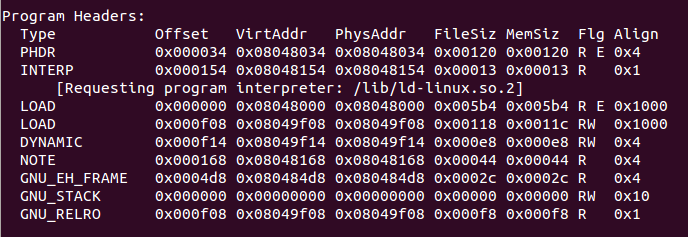
\includegraphics[width=0.85\textwidth]{figure/helloprograms.png}
  \caption{hello程序的程序头部表}
  \label{hello}
\end{figure}
%%

之所以会出现这么大的空闲地址空间,
来源于Linux(包括一些其他的UNIX)的特殊的段加载机制。
因为如果完全按照0x1000来对齐段的起始地址,
将会对物理内存产生巨大的浪费。
从图\ref{hello}可以看出,
hello程序的第一个段只有0x5b4字节大小,
让它完全占有一个物理段,那就会产生0x1000-0x5b4=0xac4字节的浪费,
空间利用率只有35.6\%。


针对这种浪费,Linux的做法是通过分配更多的虚拟内存来
换取物理内存的节约。
具体做法是把可执行文件从偏移0处开始,
按照页大小进行划分,
划分得到的每个页面作为一个物理页面加载。
这样的问题在于有的物理页面会包含两个ELF段,
这时只需要把这样的物理段映射两次到虚拟地址空间即可。
如图\ref{linuxmap},假设一个ELF文件有三个段需要加载,
在使用这种段合并机制的情况下,
三个段之间会产生两段空余的地址空间。


\begin{figure}[h!]
  \centering
  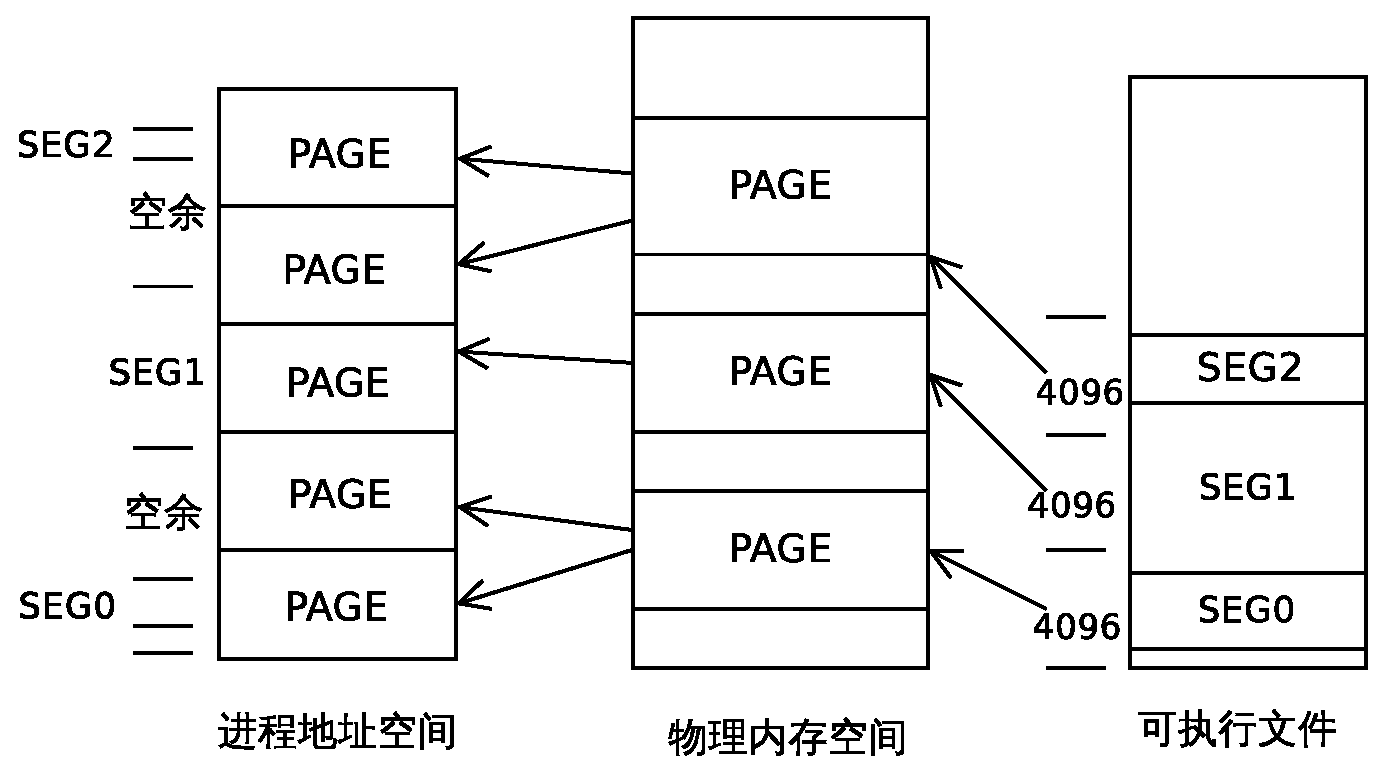
\includegraphics[width=0.65\textwidth]{figure/linuxmap.eps}
  \caption{Linux加载机制中的段合并}
  \label{linuxmap}
\end{figure}



显然,在物理地址空间中,页面利用率大幅提高,
但在虚拟地址空间中留下了尺寸不小的碎片,
图\ref{linuxmap}的情况是碎片大概1页大小,
但在有些gcc的版本中,这一大小甚至接近两个页。
这一空间便可以被我们用于插入代码。
要注意的是,虽然原理上,
数据段最后的剩余空间同样可以利用,
但这需要修改数据段的可写属性,
不如插在代码段之后更为便捷。
因此在\cite{silvio}的算法中,
代码的插入位置是在代码段之后。

下面简要描述了这一插入算法:

1、找到ELF中的第一个可加载段(代码段),
将该段的filez字段和memsz字段增加要插入代码的大小。

2、对于所有在代码段之后的段,将其offset增加一页(4KB)的大小。

3、对于代码段的最后一个节区,将其len字段增加插入代码长度大小。

4、对于在代码段之后的所有节区,将其offset字段增加一页(4KB)的大小。

5、将插入代码的长度填充到1页(4KB),然后拷贝到预定的插入代码的位置。


这一算法提出之后,大量的针对ELF乃至Linux内核的研究
都借鉴了其插入代码的思路,
如\cite{simple,prototype,subversive,cerberus,sharelib}。等

在这一算法的基础上,
我实现和完善了这一方法的python版本
(见附录\ref{python})。
并增加了一些自定义的功能。

下面借助一个例子来进一步说明其原理,
假设我们在一个ELF可执行文件中的代码段最后插入了一小段代码。
图\ref{main1}和\ref{main2}分别展示了在插入代码前后的程序头表的变化。
我们可以很容易在这里发现一些上面的算法所描述的改变,
例如第一个LOAD段的长度被增加了0x26,
而从第二个LOAD段开始,所有的段的偏移量都增加了0x1000,即4K等。
类似地,节区头部表中的一些数据结构也被修改,在此就不再赘述了。

\begin{figure}[h!]
  \label{main}
   \centering
  \begin{tabular}{cc}
    \subfigure[插入前]{
      \label{main1}
      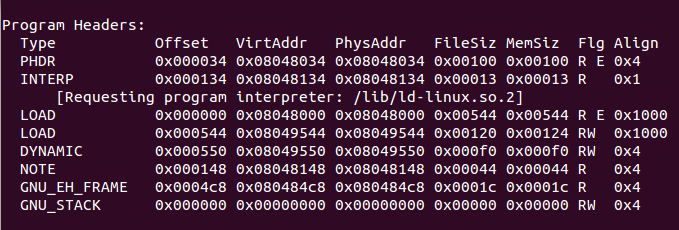
\includegraphics[width=0.85\textwidth]{figure/main.png}
     }  \\
    \subfigure[插入后]
     {
        \label{main2}
      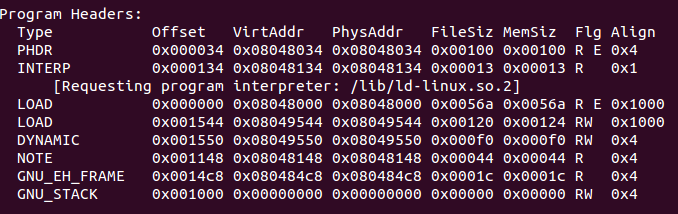
\includegraphics[width=0.85\textwidth]{figure/main2.png}
     }
    \end{tabular}
  \caption{可执行文件插入代码前后的程序头表对比}
\end{figure}
          



%%%%%%%%%%%%%%%  2.3.3 %%%%%%%%%%%%%%%%%%%%%%%%

\subsection{在代码段之前插入代码}
\label{before}

虽然利用代码段最后可能空余的地址空间来插入代码,
已经成为了一种比较成熟的手段,
但这种方法的局限性仍然是不可忽视的。
最重要的一点就是其插入的代码量存在限制。
一般来说,如果插入代码量最好保证在1KB之内,
一旦超过2KB,几乎是不可能成功的。

然而,一个高效而便捷的工具ELFsh\upcite{elfsh}
提供了一种新的插入思路,
即把代码插入至代码段之前。
我们知道,对于一个运行在IA32上的Linux系统来说,
一个进程的地址空间中,代码段总是开始于0x8048000,
然而从0到0x8047fff这段空间一般不被使用。
该工具的思路就是把需要执行的代码插入至
这一段未被使用的地址空间中。

ELFsh工具功能强大,
它以一个.o文件和一个可执行文件作为输入。
不但能够讲.o中的可执行代码插入至可执行文件中,
还能插入.o文件携带的数据节、bss节和符号表。
并能够对插入代码的所有重定位入口进行重定位。

下面简要说明其插入流程:

1、将.o文件的.bss节插入合并到可执行文件的.bss节中。

2、遍历.o文件的所有节区,判断是否具有以下条件
\begin{itemize}
  \item 存在标志位(说明该节区需要被加载到进程空间中)
  \item 在文件中占据空间(排除.bss节区)
  \item 节区类型为值为SHT\_PROGBITS,说明该节区为程序节或者代码节。
\end{itemize}
  
对于同时满足这些条件的节区,再判断节区是否具有可写属性,
对于具有可写属性的节区(数据节),插入到.bss节之后;
其他节区插入到第一个节区之前。

3、把.o文件的符号表合并至可执行文件中。

4、对于.o文件中的所有节区,如果已经被
插入到了可执行文件中,并且需要重定位,
则对其进行重定位。

下面演示ELFsh工具的效果。
我们首先编写一个简单的程序,
源代码见\ref{myprintf.c},
然后把它编译为myprintf.o即可。
我们将其注入到ls程序中。

\begin{lstlisting}[
  language={C},
  caption={myprintf.c源代码},
  label={myprintf.c},
]
#include<stdio.h>
void myprintf(){
    printf("hi, you're hijacked!");
}
\end{lstlisting}

图\ref{111}和\ref{222}反映了ls程序被插入前后的节头表(只展示了前20个)
和程序头表的变化。
由图可以发现,在ELFsh向可执行文件注入了9个节区,
并都位于可执行文件的第一个节区,即.interp节之前。
(此外还进行了符号表和.bss节的合并,这里看不出来)。
程序头表方面,可以发现段的数目并没有变化,
但是第一个段的起始地址由0x8048000提前到了0x803c000,
这也说明注入的代码使用了0x8048000之前的地址空间。
此外,位于后面的段在文件中的偏移也相应地增加了0xc000,
说明我们在.interp段之前总共插入了0xc000字节的代码,
即12个页,
试想一下,如果使用nop插入或者插入到段间的空闲地址,
这几乎是不可能完成的任务。

\begin{figure}[!ht]
    \centering
    \begin{tabular}{cc}
        \subfigure[插入前节头表]{
            \label{fig-matrix-a}
            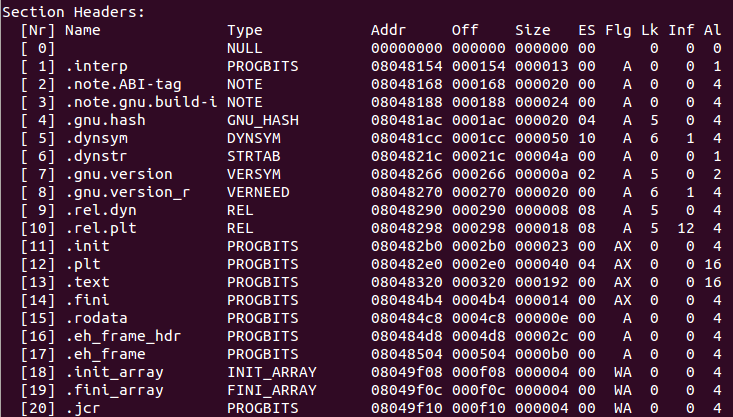
\includegraphics[width=.75\textwidth]{figure/sht1.png}
        } \\
        \subfigure[插入前程序头表]{
            \label{fig-matrix-b}
            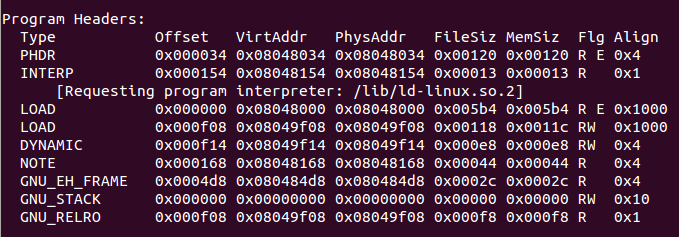
\includegraphics[width=.75\textwidth]{figure/pht1.png}
        }
       \end{tabular}
       \caption{插入前节头表与程序头表}
       \label{111}
\end{figure}



\begin{figure}[!ht]
       \centering
       \begin{tabular}{cc} 
        \subfigure[插入后节头表]{
            \label{fig-matrix-c}
            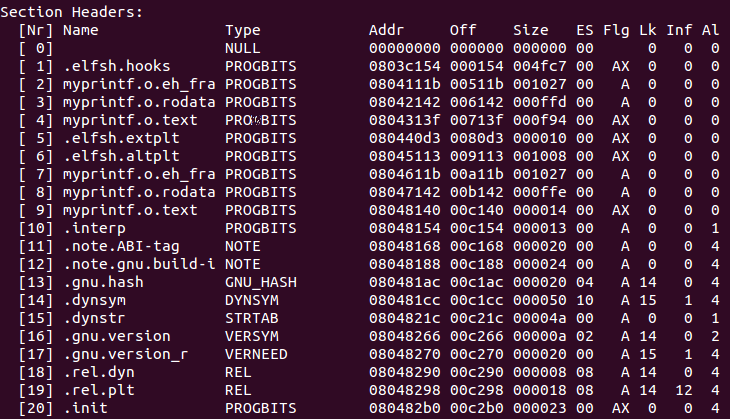
\includegraphics[width=.74\textwidth]{figure/sht2.png}
        } \\
        \subfigure[插入后程序头表]{
            \label{fig-matrix-d}
            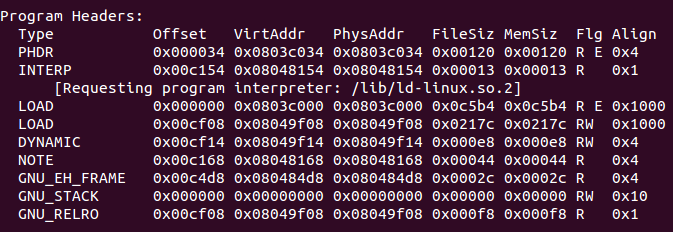
\includegraphics[width=.74\textwidth]{figure/pht2.png}
        }\\
    \end{tabular}
    \caption{插入后程序头表和节头表}
    \label{222}
\end{figure}



%%%%%%%%%%%%%%%%%%%%%%%%%%%%%%%%
%%%%%%%%%%%% 2.4 %%%%%%%%%%%%%%%
%%%%%%%%%%%%%%%%%%%%%%%%%%%%%%%%

\section{二进制程序劫持技术分析}
\label{section_hijack}

%%%%%%%%%%%%%%%%%%% 2.4.1 %%%%%%%%%%%%%%%%%%%%%%%%

\subsection{修改ELF文件入口点}

ELF文件头中包含一些有关ELF文件的重要数据结构,
一个典型的ELF文件头如图\ref{header}所示。
\begin{figure}[!ht]
  \centering
  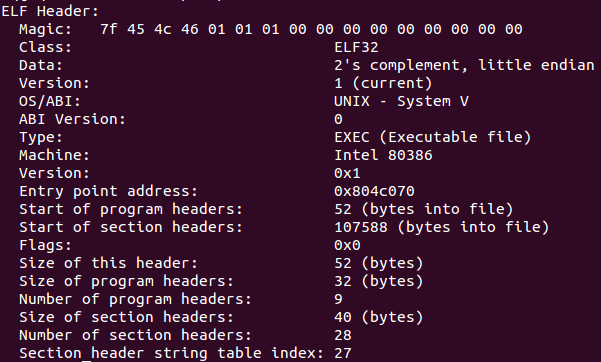
\includegraphics[width=0.75\textwidth]{figure/header.png}
  \caption{ELF文件头部}
  \label{header}
\end{figure}
文件头对于ELF文件的链接视图和执行视图来说
同样重要。除了标志该文件是ELF文件及其类型之外,
头部最重要的作用
在于标明了以下三点:

\begin{description}
  \item [1]  程序入口点位置
  \item [2]  节区头部表位置和节区的数量
  \item [3]  程序头部表位置和段的数量 
\end{description}

图\ref{header}中的“Entry Point address”即为
该ELF文件的入口点地址。
在Linux中,当ELF文件被加载完成之后,
CPU首先执行该地址处的第一条指令。
因此我们只需要修改这一地址,
就可以让系统首先跳转到我们的插入代码。

执行这一修改的步骤大致如下:

1、修改目标文件的Entry Point address字段为
插入代码第一条指令的地址。

2、插入代码执行一定的操作。

3、插入代码使用跳转指令,
跳回原入口点的地址。

这一方法简单有效,文献\cite{silvio}的第一代Unix病毒
就使用了这种办法来获取控制权。
图\ref{dia}展示了插入的代码如何通过修改程序入口点
对程序原有的正常执行流进行篡改。
在程序未被修改前,
ELF头的入口点指向代码段的起始位置,如图\ref{dia1}。
通过修改ELF头的入口点,
使它指向我们插入代码的位置;
在插入代码的最后,跳转回原入口点的位置,
以保证程序的正常执行,如图\ref{dia2}。

\begin{figure}[h!]
   \centering
  \begin{tabular}{cc}
    \subfigure[]{
      \label{dia1}
      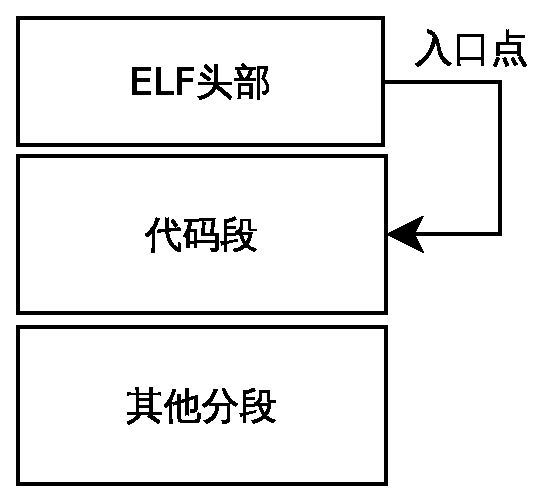
\includegraphics[width=0.27\textwidth]{figure/dia1.eps}
     }  
    \hspace{4em}
    \subfigure[]
     {
        \label{dia2}
      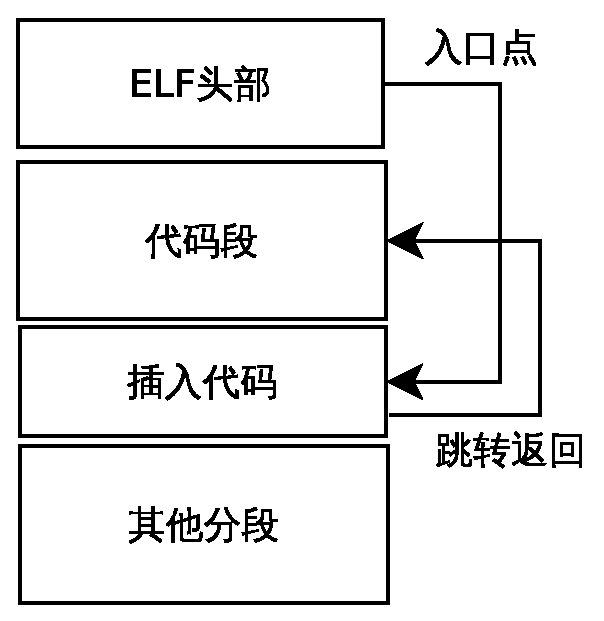
\includegraphics[width=0.3\textwidth]{figure/dia2.eps}
     }
    \end{tabular}
  \caption{可执行文件代码插入前后执行流程对比}
  \label{dia}
\end{figure}

借助\ref{before}中的例子,我们演示一下使用修改入口点进行劫持的效果。
在完成插入后,我们只需要手动修改入口点地址,指向myprintf函数即可。
然后手动修改该函数的最后几条指令,
跳回原入口点即可。
(回想一下,函数结尾往往有nop指令串,因此这很容易实现)。

最后的达到的效果如图\ref{ls}所示。

\begin{figure}[h!]
    \centering
    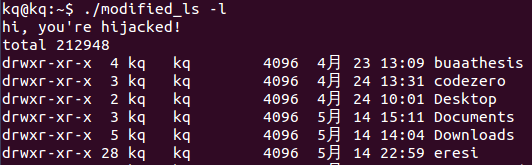
\includegraphics[width=.85\textwidth]{figure/ls.png}
    \caption{修改后的ls程序运行结果}
    \label{ls}
\end{figure}


%%%%%%%%%%%%%%%%%%%%%% 2.4.2  %%%%%%%%%%%%%%%%%%%%%%%

\subsection{在函数头增加跳转}
\label{sub_jmp}


在Linux下的ELF文件中,
我们可以通过修改ELF头部的入口点地址来实现劫持。
然而使用这种方法,
我们插入的代码将只会在程序开始时被运行一次。

我们可能不希望插入代码在
程序执行的开始就运行,
而是希望在某个函数被调用的时候,
由它来截获这一函数。
这时我们可以通过修改需要劫持的函数
的开头几条指令来进行。

下面的例子中,我们假设要劫持某个函数,
每当这个函数被调用时,都会首先输出一行“HELLO!”


一般来说,一个函数体开头的指令如代码\ref{usr}所示。

\begin{lstlisting}[
    language={[x86masm]Assembler},
    caption={函数体开头的指令},
    label={usr},
]
push ebp          
mov ebp,esp       
sub esp,0x??               
\end{lstlisting}

我们把代码\ref{usr}替换为代码\ref{inj}:

\begin{lstlisting}[
    language={[x86masm]Assembler},
    caption={函数体开头的替换指令},
    label={inj},
]
push code_address        ;压入插入代码的起始地址
ret                      ;跳转到code\_address
\end{lstlisting}


我们在适合的位置插入代码\ref{printhello},
\begin{lstlisting}[
    language={[x86masm]Assembler},
    caption={用于劫持某个函数的插入代码},
    label={printhello},
]
push ebp
mov ebp,esp
sub esp,0x??            ;补上被劫持函数的开头被修改的三条指令
push 0x000a214f
push 0x4c4c4548         ;压入字符串“HELLO!\textbackslash n”的ASCII码
push esp                ;压入字符串的起始地址。  
mov eax,0x????????      ;把printf函数的地址放入eax中
call eax                ;调用printf函数
add esp,0x8             ;恢复堆栈
push 0x????????        
ret                     ;返回被劫持函数第四条指令处。
\end{lstlisting}

这里的重点不在于我们插入的技术有多么先进,
而是插入的代码提供了一种通用的劫持任意函数的方法。
即无论我们在何种位置插入代码来劫持任意一个函数,
总是可以通过以下几个步骤来劫持一个函数的入口:

1、修改函数的前三条指令(一般为6个字节)
为push和ret(刚好也是6个字节),类似代码\ref{inj},
压栈的内容为插入代码的地址,即nop\_address。

2、插入代码的前三条指令为1中被修改的三条指令。

3、在插入代码中进行操作。

4、恢复寄存器和堆栈(如果被修改过的话)。

5、使用push+ret组合返回被被劫持函数原来的第四条指令处,
即被劫持函数地址+6。


%%%%%%%%%%%%%%%%%%%%%%  2.4.3 %%%%%%%%%%%%%%%%%%%%%%  

\subsection{通过篡改动态链接数据结构}
\label{sub_plt}

ELF中文件关于动态链接的细节,
应参见\cite{elf1.2},
然而,本条中讲述的劫持方法,
不但简单明了,而且像教科书一般阐明了ELF中
对动态库函数的引用机制。

动态链接的ELF可执行文件中,
所有对于外部库函数的调用,都是通过
一个got数据结构和一个段plt代码来实现的。


为了实现对外部函数引用的劫持工作,
需要我们插入两段代码:
A段在函数入口点处执行,作用是帮助我们修改got,
定位到插入库函数的位置。
B段则是我们插入的库函数。
这两段代码的插入可以用上一节中描述的三种方法
的任意一中来进行。

两段代码的算法简要描述如下:

A:

1、使用系统调用,为代码段增加可写属性。

2、保存got中对应条目的地址,记为original\_got。

3、将got中条目的地址修改为插入的库函数的地址。

B:

1、执行目的操作,例如打印一行信息。

2、恢复got中旧的条目的地址。

3、恢复堆栈,调用原库函数。

4、保存got中的地址,覆盖original\_got。

5、将got中的地址替换为插入的库函数的地址。

在B代码的第4步要重新保存一遍original\_got,
因为动态链接程序大都是用“延迟绑定”机制,
在第一次调用库函数时,
会经过plt进行一次间接跳转,
并会调用动态链接器进行重定位,
从而修改got中保存的地址。




















